%!TEX root = ../main.tex
%%%%%%%%%%%%%%%%%%%%%%%%%%%%%%%%%%
% Links:
%
% Difficulty:
% Companies: 
%%%%%%%%%%%%%%%%%%%%%%%%%%%%%%%%%%

\chapter{$n^{th}$ node from the end}
\label{ch:node_from_the_end}
\section*{Introduction}
The problem presented in this chapter is a particularly interesting one on Linked List. It has been asked numerous times in companies like Amazon and Google and it is therefore important that we understand and master the solution to this problem.

\section{Problem statement}
\begin{exercise}
Given a linked list $L$ (which definition is shown in Listing \ref{list:delete_duplicates_list:linked_list} at page \pageref{list:delete_duplicates_list:linked_list} , and an integer $n$ remove the $n^{th}$ node from the end of list.

\begin{example}
	\hfill \\
	Given $L=[1,2,3,4]$, and $n=2$ the function returns: $L=[1,2,4]$. See Figure \ref{fig:node_from_the_end:example1}.
\end{example}

\begin{example}
	Given $L=[1,2,3,4]$, and $n=0$ the function returns: $L=[1,2,4]$.
	See Figure \ref{fig:node_from_the_end:example2}.
\end{example}
\end{exercise}


\begin{figure}
	\label{fig:node_from_the_end:example1}
	\centering
	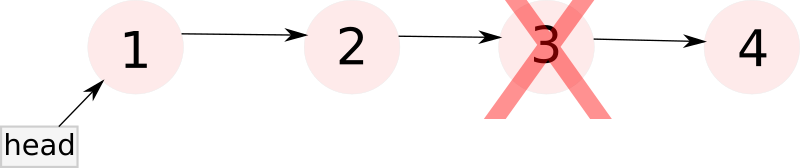
\includegraphics[scale=1.0]{sources/node_from_the_end/images/example1}
	\caption{Removal of the \nth{2} to last element in a singly linked list of length $4$.}
\end{figure}

\begin{figure}
	\label{fig:node_from_the_end:example2}
	\centering
	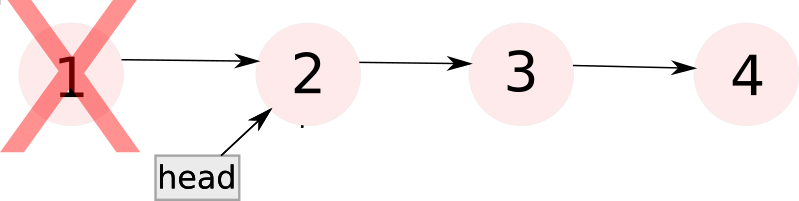
\includegraphics[scale=1.0]{sources/node_from_the_end/images/example2}
	\caption{Removal of the \nth{4} to last element in a singly linked list of length $4$. The head pointer needs to be updated.}
\end{figure}


\section{Clarification Questions}

\begin{QandA}
	\item \begin{questionitem} \begin{question} Is $n$ guaranteed to be a valid node in the list?  \end{question} 	 
    \begin{answered}
		\textit{Yes you can assume that $n$ is the index of a valid node in the list.}
	\end{answered} \end{questionitem}
\end{QandA}

\section{Discussion}
\label{node_from_the_end:sec:discussion}
This problem has two main parts in it: 
\begin{enumerate}
	\item Finding out the index of the $n$-to last node
	\item Removing a node from the list
\end{enumerate}
Those tasks are separate and thus we can solve each of them separately and then use the solution to these two subproblems to obtain our final answer.

\subsection{Brute-force}
\label{node_from_the_end:sec:bruteforce}
Finding out the the node to be deleted becomes trivial once we know how long the list is. Therefore the brute-force approach simply performs a first pass in the list and counts how many nodes it is made of i.e. $l$. Then it performs another pass but it stops at node $l-n$ (the n-to-last node) and removes it.
Please note that in order to correctly remove a node from a singly linked list a we need to have a pointer to the node we want to remove as well as a pointer to its predecessor (variable \inline{pred} in the code). This approach can be implemented as shown in Listing \ref{list:node_from_the_end:bruteforce}, and it has a time and space complexity of  $O(n)$ and $O(1)$, respectively.


\lstinputlisting[language=c++, caption={Sample Caption},label=list:node_from_the_end:bruteforce]{sources/node_from_the_end/node_from_the_end_solution1.cpp}

\subsection{Two pointers}
\label{node_from_the_end:sec:twopointers}
There is however another way of solving this problem that is our opinion is slightly better even if it is not in terms of asymptotic complexity. 
The key issue we have with this problem is that we have to delete a node at index $l-n$ but we have no idea what $l$ is and we do not want to compute it explicitly. 
What we can do it to loop forward with a pointer $s$ from the head of the list for $n$ nodes. At this point $s$ will be at $n$ node distance from the head and at $l-n$ from the tail. We now have a way of counting $n-l$. Let $f$ be a pointer to the head of the list: we can advance both $f$ and $s$ until $s$ reaches the end of the list. At that point $s$ had advanced $l-n$ times and $f$, crucially will be pointing at the node $l-n$ i.e. at the n-to-last node.

This idea is implemented in Listing \ref{list:node_from_the_end:twopointers}. Please note that the second \inline{while}, as in the brute-force approach (Listing \ref{list:node_from_the_end:bruteforce}) also need to keep a pointer to the node proceeding the one that needs to be deleted (pointer $p$ in the code).

The complexity of this implementation is linear in time and constant in space.


\lstinputlisting[language=c++, caption={Sample Caption},label=list:node_from_the_end:twopointers]{sources/node_from_the_end/node_from_the_end_solution2.cpp}

\subsection{Common Variation}
\subsubsection{List midpoint}
\label{node_from_the_end:sec:list_midpoint}

\begin{exercise}
Given a linked list $L$ of length $l$ (which definition is shown in Listing \ref{list:delete_duplicates_list:linked_list} at page \pageref{list:delete_duplicates_list:linked_list} , return the value of the node at position $\frac{l}{2}$.
\begin{example}
	\hfill \\
	Given $L=[1,2,3,4]$, the function returns $2$.
\end{example}

\begin{example}
	Given $L=[1,5,7,8,9,4,5,6,1,2,4,9,7]$, the function returns $5$.
\end{example}
\end{exercise}
This is a very popular variation of the problem described in this chapter. It can be solved using the same methods described in Sections \ref{node_from_the_end:sec:bruteforce} and \ref{node_from_the_end:sec:twopointers} or using an ad-hoc(spoiler: a fast and a slow pointers